\begin{figure}[h]
    \centering
    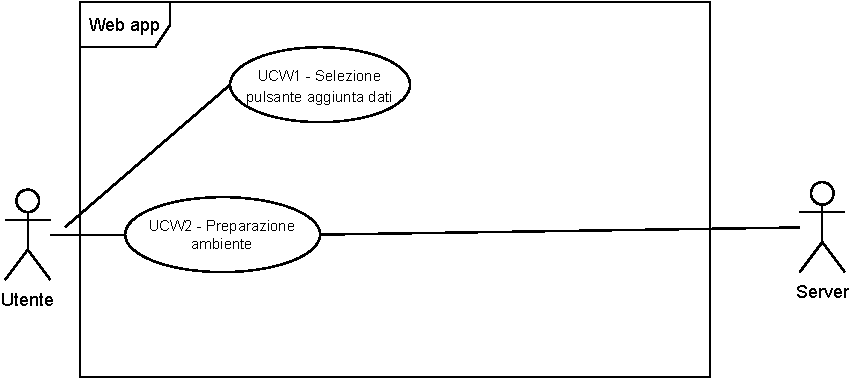
\includegraphics[width=0.7\textwidth]{diagrammi/UC0.pdf}
    \caption{Diagramma rappresentante UCW1 e UCW2}
    \label{fig:UCW0}
\end{figure}

\subsection{UCW1 - Selezione opzione aggiunta dati}
\label{sub:ucw1}

\begin{itemize}
    \item \textbf{Descrizione}: L'utente prepara seleziona l'opzione di aggiunta dei dati.

    \item \textbf{Attore primario}: Utente;

    \item \textbf{Precondizione}:   L'applicazione è in esecuzione;

    \item \textbf{Postcondizione}:  Viene selezionata l'opzione di aggiunta dei dati;

    \item \textbf{Scenario principale}:
          \begin{enumerate}
              \item L'utente seleziona l'opzione di aggiunta dei dati;
          \end{enumerate}

\end{itemize}

\subsection{UCW2 - Preparazione ambiente}
\label{sub:ucw2}

\begin{itemize}
    \item \textbf{Descrizione}: L'utente prepara l'applicativo HD Viz alla visualizzazione dei dati selezionando la fonte del suo dataset.

    \item \textbf{Attore primario}: Utente;

    \item \textbf{Precondizione}:   L'utente ha selezionato l'opzione di aggiunta dei dati (\hyperref[sub:ucw1]{UCW1});

    \item \textbf{Postcondizione}:  Viene selezionata la fonte dei dati desiderata;

    \item \textbf{Scenario principale}:
          \begin{enumerate}
              \item L'utente seleziona l'opzione di aggiunta dei dati;
              \item L'utente seleziona la fonte dei dati da importare;
          \end{enumerate}

\end{itemize}

\begin{figure}[h]
    \centering
    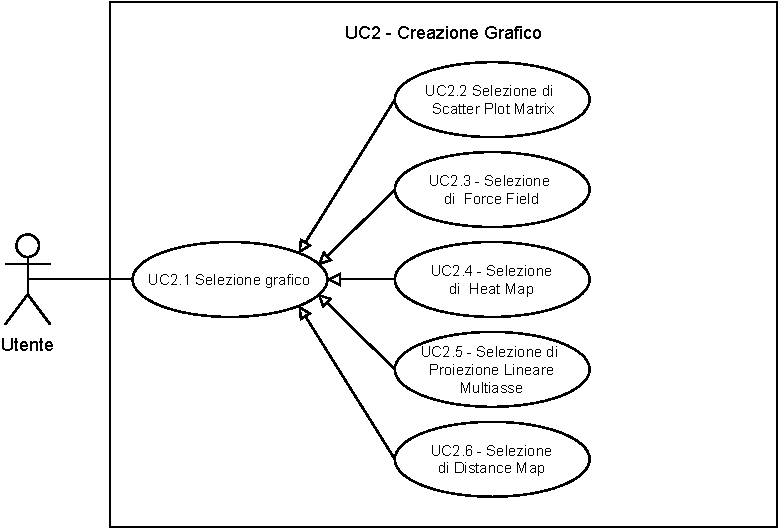
\includegraphics[width=0.7\textwidth]{diagrammi/UC2.pdf}
    \caption{Diagramma rappresentante UCW2}
    \label{fig:UCW2}
\end{figure}

\subsubsection{UCW2.1 - Selezione fonte}
\label{ssub:ucw2.1}
\begin{itemize}
    \item \textbf{Descrizione}: L'utente decide di impostare l'ambiente scegliendo la fonte di un dataset;

    \item \textbf{Attore primario}: Utente;

    \item \textbf{Precondizione}:   L'applicazione è in esecuzione;

    \item \textbf{Postcondizione}:  Viene selezionata la fonte del dataset;

    \item \textbf{Scenario principale}:
          \begin{enumerate}
              \item L'utente seleziona l'opzione di aggiunta dei dati:
          \end{enumerate}

    \item \textbf{Generalizzazioni}:
          \begin{enumerate}
              \item Selezione dell'opzione file csv (\hyperref[ssub:ucw2.2]{UCW2.2});
              \item Selezione dell'opzione database (\hyperref[ssub:ucw2.3]{UCW2.3}).
          \end{enumerate}
\end{itemize}


\subsubsection{UCW2.2 - Selezione del file csv}
\label{ssub:ucw2.2}
\begin{itemize}
    \item \textbf{Descrizione}: L'utente seleziona un file csv del suo dispositivo;

    \item \textbf{Attore primario}: Utente;

    \item \textbf{Precondizione}:   L'applicazione è in esecuzione;
    \item \textbf{Postcondizione}:  Viene selezionato un file csv;

    \item \textbf{Scenario principale}:
          \begin{enumerate}
              \item L'utente seleziona l'opzione di aggiunta dei dati mediante file;
              \item L'utente seleziona il file csv di dati da importare.
          \end{enumerate}
\end{itemize}

\subsubsection{UCW2.3 - Selezione del database}
\label{ssub:ucw2.3}
\begin{itemize}
    \item \textbf{Descrizione}: L'utente seleziona l'input da database e un file di configurazione;

    \item \textbf{Attore primario}: Utente;

    \item \textbf{Precondizione}:   L'utente decide di caricare i dati mediante un database;
    \item \textbf{Postcondizione}:  Viene selezionato l'input da database e la configurazione desiderata;

    \item \textbf{Scenario principale}:
          \begin{enumerate}
              \item L'utente seleziona l'input da database;
              \item L'utente seleziona una delle impostazioni di configurazione predefiniti.
          \end{enumerate}

\end{itemize}
